\documentclass[10pt,twocolumn,oneside]{article}
\setlength{\columnsep}{10pt}                    %兩欄模式的間距
\setlength{\columnseprule}{0pt}                 %兩欄模式間格線粗細

\usepackage{amsthm}								%定義,例題
\usepackage{amssymb}
\usepackage{fontspec}							%設定字體
\usepackage{color}
\usepackage[x11names]{xcolor}
\usepackage{listings}							%顯示code用的
\usepackage{fancyhdr}							%設定頁首頁尾
\usepackage{graphicx}							%Graphic
\usepackage{enumerate}
\usepackage{titlesec}
\usepackage{amsmath}
\usepackage[CheckSingle, CJKmath]{xeCJK}
 \usepackage{CJKulem}
\usepackage{tikz}
\usepackage{amsmath, courier, listings, fancyhdr, graphicx}
\topmargin=0pt
\headsep=5pt
\textheight=740pt
\footskip=0pt
\voffset=-50pt
\textwidth=545pt
\marginparsep=0pt
\marginparwidth=0pt
\marginparpush=0pt
\oddsidemargin=0pt
\evensidemargin=0pt
\hoffset=-42pt

%\renewcommand\listfigurename{圖目錄}
%\renewcommand\listtablename{表目錄}

%%%%%%%%%%%%%%%%%%%%%%%%%%%%%

\setmainfont{Consolas}
%\setmonofont{Ubuntu Mono}
\setmonofont{Consolas}
\setCJKmainfont{Noto Sans CJK TC}
\XeTeXlinebreaklocale "zh"						%中文自動換行
\XeTeXlinebreakskip = 0pt plus 1pt				%設定段落之間的距離
\setcounter{secnumdepth}{3}						%目錄顯示第三層

%%%%%%%%%%%%%%%%%%%%%%%%%%%%%
\makeatletter
\lst@CCPutMacro\lst@ProcessOther {"2D}{\lst@ttfamily{-{}}{-{}}}
\@empty\z@\@empty
\makeatother
\lstset{										% Code顯示
    language=C++,									% the language of the code
    basicstyle=\footnotesize\ttfamily, 					% the size of the fonts that are used for the code
    %numbers=left,									% where to put the line-numbers
    numberstyle=\footnotesize,					% the size of the fonts that are used for the line-numbers
    stepnumber=1,									% the step between two line-numbers. If it's 1, each line  will be numbered
    numbersep=5pt,									% how far the line-numbers are from the code
    backgroundcolor=\color{white},				% choose the background color. You must add \usepackage{color}
    showspaces=false,								% show spaces adding particular underscores
    showstringspaces=false,						% underline spaces within strings
    showtabs=false,								% show tabs within strings adding particular underscores
    frame=false,										% adds a frame around the code
    tabsize=2,										% sets default tabsize to 2 spaces
    captionpos=b,									% sets the caption-position to bottom
    breaklines=true,								% sets automatic line breaking
    breakatwhitespace=false,						% sets if automatic breaks should only happen at whitespace
    escapeinside={\%*}{*)},						% if you want to add a comment within your code
    morekeywords={*},								% if you want to add more keywords to the set
    keywordstyle=\bfseries\color{Blue1},
    commentstyle=\itshape\color{Red4},
    stringstyle=\itshape\color{Green4},
}


\begin{document}
\pagestyle{fancy}
\fancyfoot{}
%\fancyfoot[R]{\includegraphics[width=20pt]{ironwood.jpg}}
\fancyhead[C]{National Central University}
\fancyhead[L]{NekoCuteUwU}
\fancyhead[R]{(\today) \thepage}
\renewcommand{\headrulewidth}{0.4pt}
\renewcommand{\contentsname}{Contents}

\scriptsize
\tableofcontents
\section{Basic}
	\subsection{vimrc}
			\lstinputlisting{Basic/vimrc}
	\subsection{Python stress}
			\lstinputlisting{Basic/stress/py.py}	
	
	\subsection{C++ stress}
			\lstinputlisting{Basic/stress/cpp.cpp}	
\newpage			
\section{Graph}
	\subsection{DSU}
		\lstinputlisting{Graph/DSU.cpp}
	\subsection{LCA}
		\lstinputlisting{Graph/LCA.cpp}
		
\section{Flow}
	\subsection{Dinic}
		\lstinputlisting{Graph/Flow/dinic.cpp}
	\subsection{MinCostFlow}
		\lstinputlisting{Graph/Flow/MinCostFlow.cpp}
		
\section{Matching}
	\subsection{KM}
		\lstinputlisting{Graph/Matching/Kuhn_Munkres.cpp}
		
\section{Geometry}
		\subsection{ConvexHull}
		\lstinputlisting{Geometry/Convex_Hull.cpp}

\section{Tree}
		\subsection{Trie}
		\lstinputlisting{Tree/Trie.cpp}
				
\section{Math}
		\subsection{Miller Rabin}
		\lstinputlisting{Math/Miller_Rabin.cpp}
		\subsection{Josephus Problem}
		\lstinputlisting{Math/Josephus_Problem.cpp}
		\subsection{Phi}
		\lstinputlisting{Math/Phi.cpp}
		
\section{Data Structure}
		\subsection{區間修改線段樹}
		\lstinputlisting{DataStructure/segmentTree_segmentModify.cpp}
		\subsection{pbdsKth}
		總共有$n$件衣服,各自有不同的價格$(a_1, a_2, ..., a_n)$。\\
一開始第$i$件會在編號為$i$的桶子裡,接下來會有$m$筆操作\\
每次操作有三種選擇:\\
- A x y :將編號第$x$的衣服所在桶子裡面所有的衣服,倒到第$y$件衣服所在的桶子 $(1 ≤ x, y ≤ n)$\\
- M x y :第$x$件衣服的售價改為$y (1 ≤ x ≤ n, 1 ≤ y ≤ 10^9)$\\
- Q x y :查詢第$x$件衣服所在的桶子,裡面第$y$大的售價 $(1 ≤ x ≤ n)$\\
\\
$1 ≤ n ≤ 10^5$\\
$1 ≤ m ≤ 4 * 10^5$\\
\\
5 4\\
7 8 5 13 12\\
Q 4 1\\
A 5 4\\
A 3 4\\
Q 4 3\\
\\
13\\
5\\
		\lstinputlisting{DataStructure/pbds_kth.cpp}
		
\section{Other}
		\subsection{Suifeng0214}
		\lstinputlisting{Other/suifeng0214.cpp}
		\subsection{Xiang1078}
		\lstinputlisting{Other/xiang1078.cpp}
		
\onecolumn
\centering
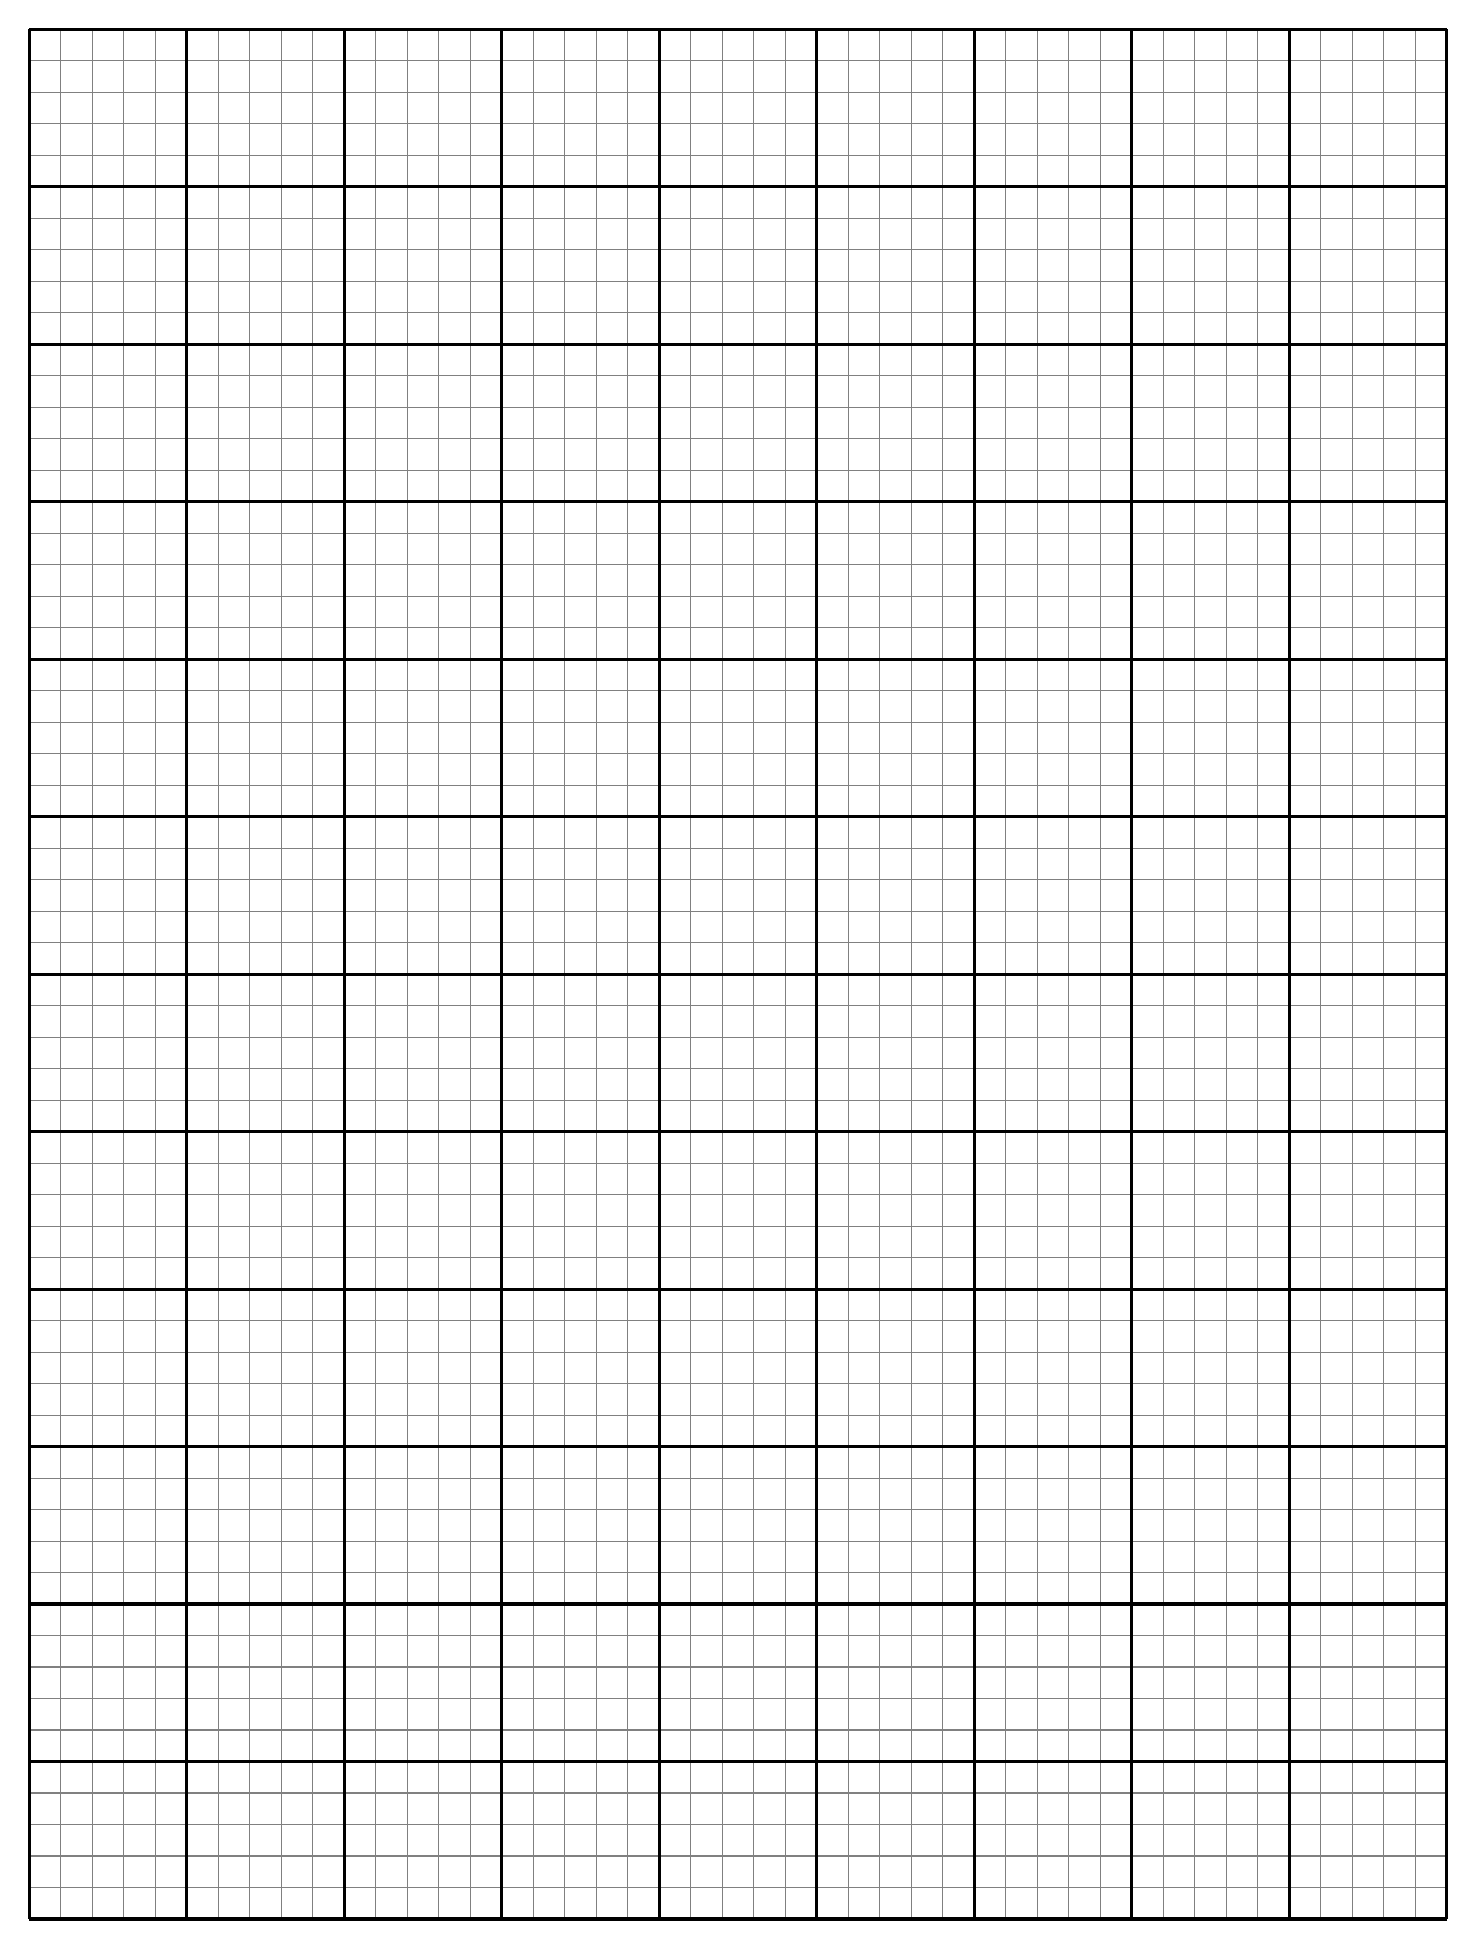
\begin{tikzpicture}[every node/.style={minimum size=1cm-\pgflinewidth, outer sep=10pt}, scale=2]
    \draw[step=0.2cm,color=gray] (0,0) grid (9,12);
    \draw[step=1cm,color=black,line width=0.4mm] (0,0) grid (9,12);
\end{tikzpicture}

\centering
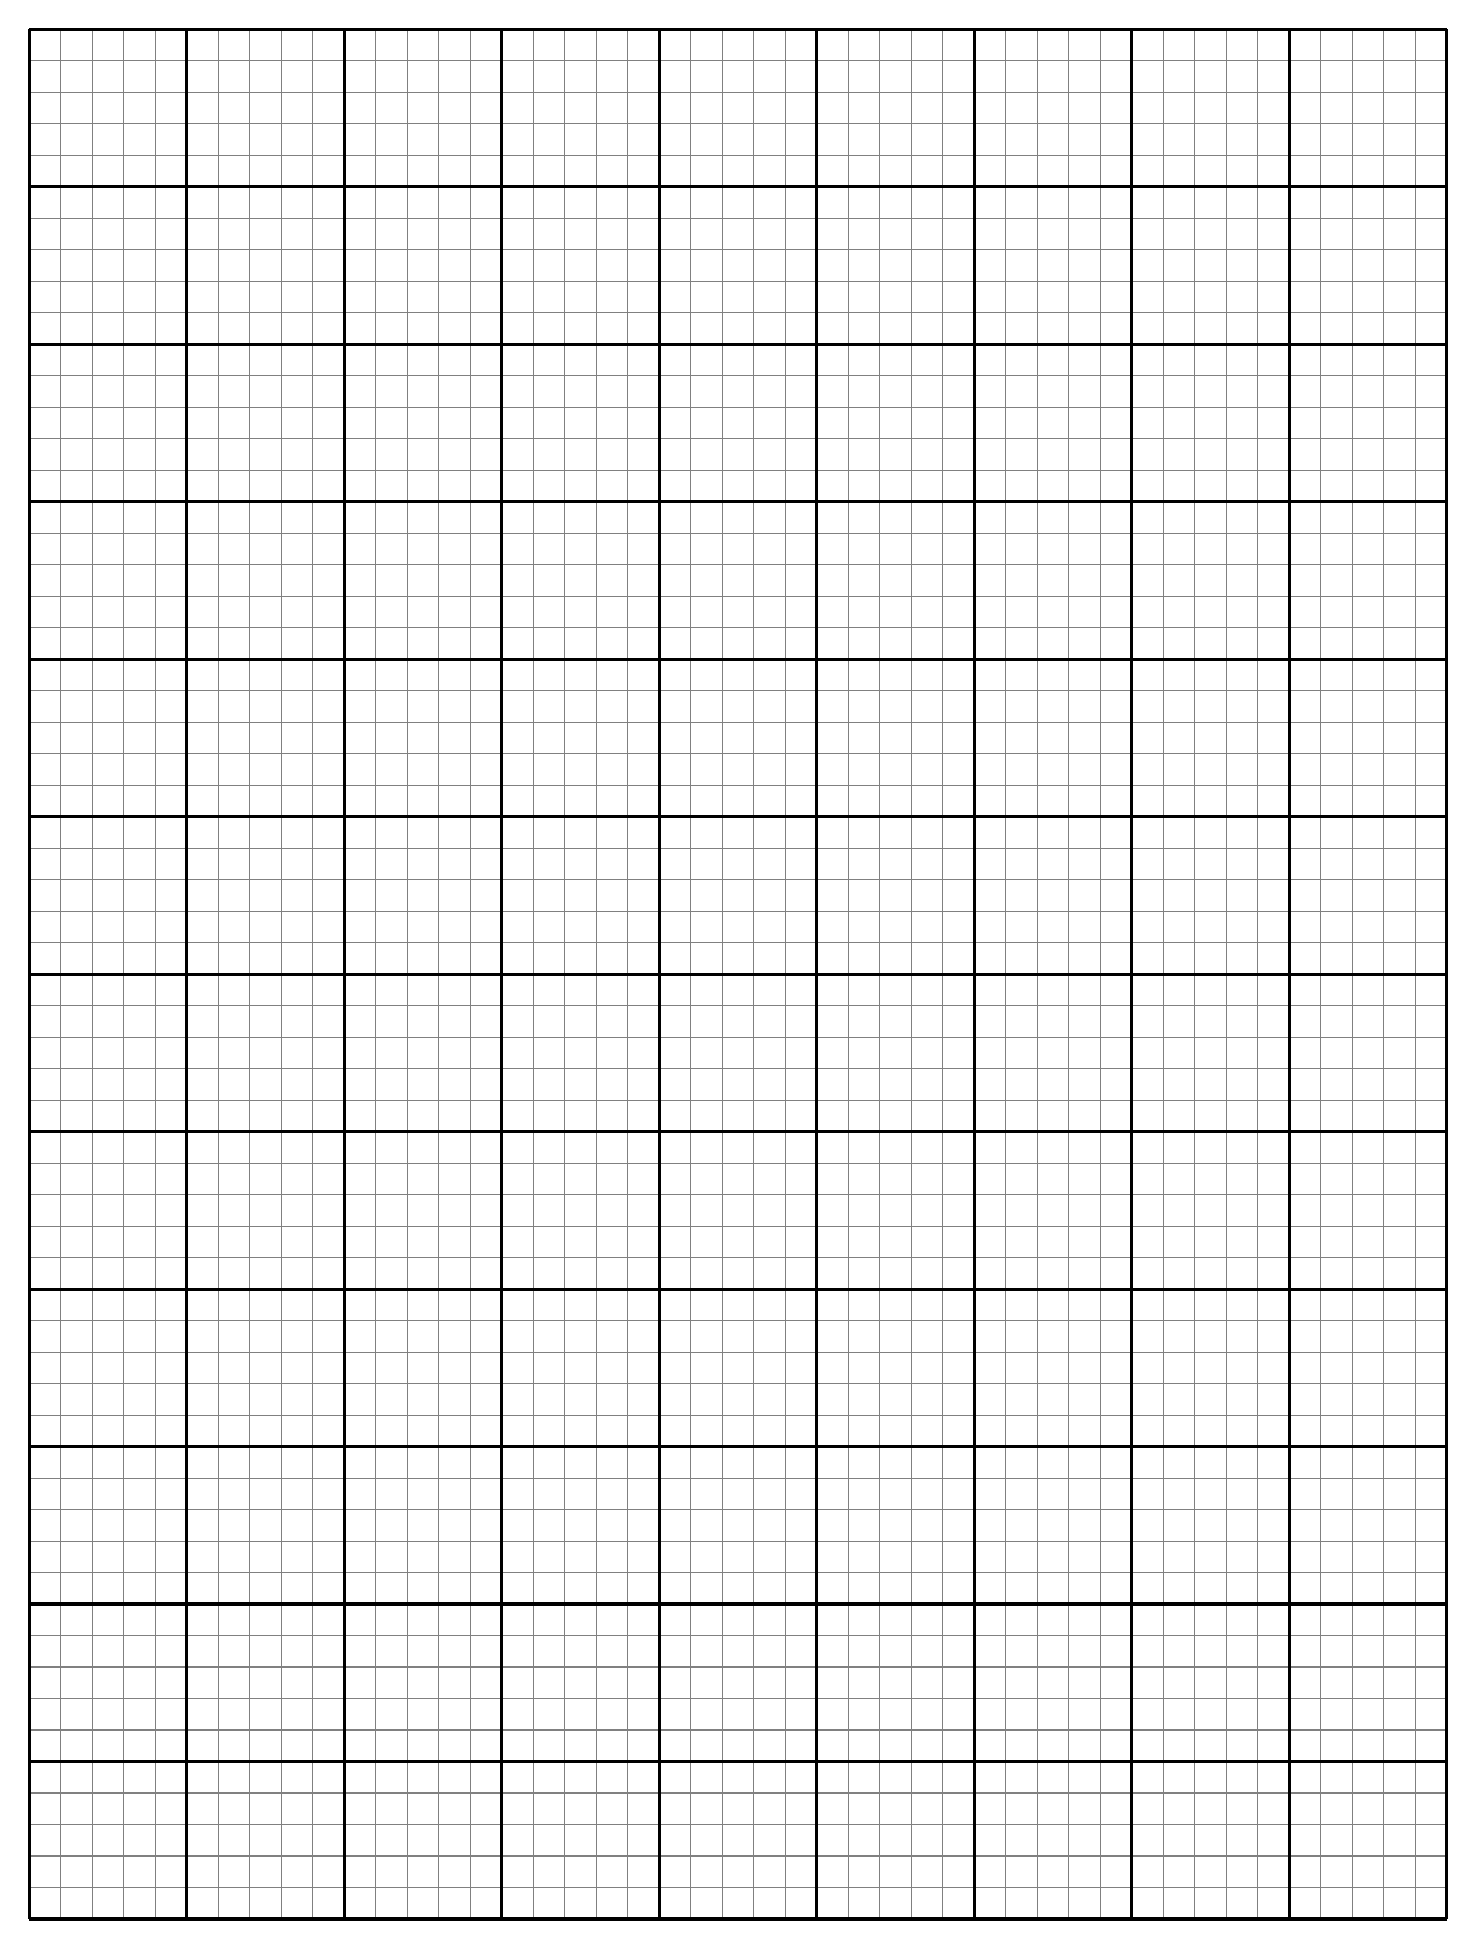
\begin{tikzpicture}[every node/.style={minimum size=1cm-\pgflinewidth, outer sep=10pt}, scale=2]
    \draw[step=0.2cm,color=gray] (0,0) grid (9,12);
    \draw[step=1cm,color=black,line width=0.4mm] (0,0) grid (9,12);
\end{tikzpicture}
\newpage
\section{Empty}
\newpage
\section{Empty}
\newpage
\section{Empty}

\end{document}